\section{Behavior Selection Through Reinforcement Learning}
Due to the challenges using orthodox method, in this paper, for robot to behave according to the applied force, we used reinforcement learning to estimate the intention of the applied force as describe in figure \ref{fig:end}. This method eliminates the need to recognize external force and plan behavior manually. Instead, we �etrain/teach�f the robot, in a manner similar to how father �etrain/teach�f their child, intuitively without scientific background requirement.

\begin{figure}[!h]
\begin{center}
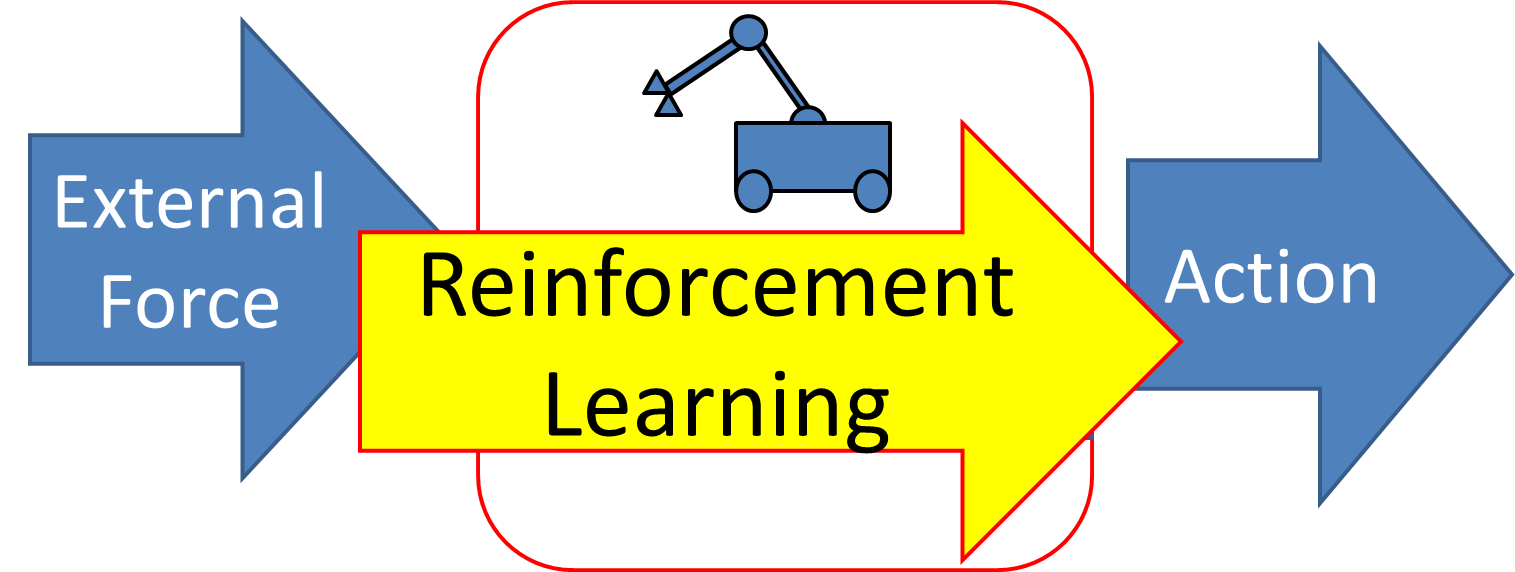
\includegraphics[width=9cm]{end_method.png}
\caption{end-to-end method}
\label{fig:end}
\end{center}
\end{figure}

Learning in reinforcement learning is accomplished by selecting behaviors to maximize the reward. Given the state $s$ in time step $t$, an agent seeks to execute action $a$ to maximize the reward $r$ which is define by $R_t=��_{\tau=t}^{��} \gamma^{\tau-t} r_\tau$ where $\gamma��[0,1]$ is a discount factor that trades-off priority of immediate and future rewards. Further introduction can be found in \cite{sutton}.

\subsection{Deep Q Network}
To handle high dimension input, this paper uses neural network to approximate using deep Q network \cite{mnih}, $Q(s,a;\theta)$ with parameters $\theta$ using the following Q-learning algorithm:

\begin{equation}
Target=r+\gamma maxQ(s',a';Q^{-})
\end{equation}

In reinforcement learning, approximating nonlinear function such as neural network are difficult to do as it is generally unstable and diverges. This however can be overcome using two key ingredient, experience replay and target network as describe in \cite{mnih}. \\

\subsection{Double Deep Q Network}
In this paper, it is planned to use the Double DQN (DDQN) reinforcement learning algorithm proposed by \cite{van}. The Q-Learning algorithm and the conventional DQN algorithm uses the max operators to estimate the true value. However, this tends to overestimates the optimal value as describe in \cite{van}. To overcome this problem, DDQN uses the following algorithm:
\begin{equation}
Target=r+\gamma Q(s',argmax(Q(s',a';\theta_{i});Q^{-})
\end{equation}